While our ICCAD 2019 publication focussed on how to flexibly introduce resource
optimizations without changing target behavior, our rework of MIDAS's endpoint
system was the second major development in the compiler and was implemented in
the months thereafter. If Golden Gate is to FPGA hosts as verilator or VCS is
to CPU hosts, then target-to-host Bridges can be best thought of as Golden
Gate's analog of the Verilog Procedural Interface~(VPI): they provide a
side-channel mechanism for the user to inject arbitrary, often unsynthesizable
modeling resources anywhere in their design. In practise, many features
implemented using VPI can re-implemented for FireSim using bridges: the
black-box wrapping a VPI call can be annotated as a bridge. When the design is
simulated in a conventional RTL simulator the VPI implementation used, when it
is simulated in FireSim its bridge implementation is used.

Bridges serve the same purpose as endpoints but differ in three primarys ways:
\begin{enumerate}
    \item They are integrated into the target as modules, and elaborated as
        part of the target.  Bridges can be instantiated at any level in the
        design hierarchy, not simply in the top level.  So while Bridges can be
        used like endpoints to provide I/O models for the dut, they enable many
        other applications: They can be used to instantiate units that serve as
        monitors or golden models, to verify parts of the target in-situ. They
        can be used to provide alternate implementations of expensive or
        unsynthesizable target modules deep in the module hierarchy. This
        provides a second means to introduce resource optimizations.


    \item Their elaboration-time parameters are serializable. This permits elaborating 
        the target in a separate process to golden-gate invocation.

    \item They can easily parameterized by their instantation context. With
        endpoints, it was difficult to disambiguate between multiple intances
        of the same type of endpoint (e.g., different channels of the sameDRAM
        subystem all appear as AXI4 interfaces on the top-level I/O). Conversly,
        when bridges are instantiated they can accept arbitrary parameters that
        may only be known at their instantiation site (e.g., the number of
        outstanding memory requests that may be made on an AXI4 interface).
\end{enumerate}

\section{Achieving Good Performance: The Crux Of Bridge Design}
Of course, to support VPI-like functionality on an FPGA is a fundamentally more
challenging prospect due primarily host-transport considerations and speeds at
which the simulator is executing. A naive bridge implementation, could reuse
same VPI source code hosted as part of a BridgeDriver, the driver could read
I/O values from the FPGA, invoke the VPI function on those values, and then
write updated values to the FPGA (the bridge Module would emit these new values
as one-or-more tokens).

Let's consider the performance of this approach for VPI call that models a
purely combinational function~(i.e., it has no target state it must update from
timestep to timestep): this represents both the simplest case to analyze and
has the worst-case simulation performance. Lets consider a simple hybrid
CPU-FPGA host system, shown in \TODO{figure}.

Where, l is the inter-FPGA-CPU transport latency, which we'll assume to be the
time required to move all bits of an input token to the CPU or all bits of the
output tokens back to the FPGA. In practise $l$ scales with the size of the
tokens due to serialization and deserialization latencies, but we'll neglect
this for now.
$p$ is the latency of invoking the function that models the
combinational function, essentially the time it takes to run code that
implements the VPI call on the host CPU.
$f$ is the period of one FPGA cycle.

FMR in this resulting system, is given \TODO{by}.

In this system, in order to maintain unity FMR, $2l + p < f$, a practical
impossiblity -- as even the time required to move the token across FPGA-fabric
will require some multiple $f$ seconds. To make this more concrete, consider
typical times on an EC2 F1 host. Empirically, we've measured MMIO read and
write latencies, specifically the latency between a BridgeDriver calls
simif\_t::write or simif\_t::read, and when that function returns as taking
\TODO{seconds} \TODO{seconds} respectively. Assuming, $f_{fpga}$ of 100 MHz, a
readily achievable frequency for multicore Rocket designs with shared L2
caches. In this case, even if we assume $p = 0$, simulator FMR must exceed
\TODO{10}.

Another artificial but illustrative case to consider is when $l = 0$, and $p$
is non-zero (this is roughly analagous to having a bridge directly connected to
the hub-unit, or using using flow-through queues as the channel implementations). Given a CPU-host frequency
of, this gives exactly \TODO{cycles} on the CPU host to model the combinational
function.

A final illustrative case to consider, is one in which a bridge is purely a
sink or source of tokens. Here there is no causal loop between parts of the
simulator hosted on the CPU and on the FPGA~(we assume no other side channels).
and the bridge can decouple arbitrarily from the the rest of the simulator.
Even still, these bridges can result in FMR penalties due to rate-limiting, if
there is insufficient bandwidth to move tokens between the FPGA and CPU. We update our model,
to suppose the host can support $K$ GB/s of read and write bandwidth.
update our model, such that such.

There is hope for the simulation designer, assuming they can exploit one of two key properties. 
The first is target latency of the underlying causal relationship.~\TODO{clocks} A combinational path is the worst case
as for the purpose of delay-less RTL simulation, as this is essentially zero. If we consider a loopback with
path with $t_l$ registers, to maintain unity FMR, our unit would need to meet:

The other properties is that often $p$ is non uniform, for many cycles, a unit
may have nothing to do here $p$ can apporach zero.  In otherwords, it might be
acceptable to model even something like a combinational function in software,
if that function is evaluated infrequently.

These analyzes become vastly more complex when accounting for variability in
host timings, non-uniform FMR introduced by other simulation components, an
contention for shared simulation resources, but it highlights \TODO{4} general
strategies for improving bridge and unit performance.

To summarize, the simulator design has four major tools they can deploy:
\begin{enumerate}
    \item Reduce $l$.
    \item Reduce $p$.
    \item Exploit or increase $t_l$.
    \item Exploit or increase $d$.
\end{enumerate}


These are not by any means new observations---they are fundamental properties
of any program running over a distributed host. Generalizations of this
analysis can be found through the distributed computing literature, especially
in PDES, where causality constraints between parts of a distributed simulation
impose a precise coupling between pieces of the simulation. Moreover, these
challenges are well known in the commercial hardware-emulation space, where
special care is given to parts of the emulator that span FPGA-and-CPU.

However, we feel it is important for bridge designers to understand the
constant factors at play (i.e., the expected latencies and bandwidths they must
design around) when writing a bridge) when designing for FireSim specifically,
and give examples of how to overcome these limitations.  To this end, we
describe three notable bridge implementations in FireSim. FESVR-over-TSI, a
low-bandwidth bridge relies on regularizing infrequent interactions;
Synthesized Printfs, a sink-only bridge, that uses FPGA-DMA to supply the need
host-bandwidth to prevent simulation stalls; and FASED memory timing models,
which uses FPGA DRAM as a backing store and attempts to hide the latency of
FPGA-DRAM access by modelling DRAM memory systems at the DRAM controller
boundary (as opposed to modelling the DRAM devices at the SoC boundary
interface).

\section{FESVR-over-TSI Bridge}
At time of writing, all target designs supplied in Chipyard (and present in
FireSim previously) are \emph{tethered}, and cannot boot standalone. The RISC-V
Frontend Server (FESVR) is responsible for managing the early stages of boot.
It keeps the target HARTs under reset, while it loads a binary into target
DRAM, (e.g., the Berkeley Boot Loader\cite{BBL} and a linux kernel, or a
baremetal binary). During execution, FESVR monitors the target by periodically
polling \texttt{tohost}. The SoC can proxy certain types of I/O, like printfs)
to FESVR, by setting tohost to a specific value, and providing an address to a
buffer that FESVR can decode and process. While we do not use these features,
since we have our own IO device models, FESVR only remaining responsibility is
to detect when an SoC has successfully "powered down", so that it may signal
the end of the simulation.

The tether-serial interface (TSI), is one transport layer implementation for
FESVR requests that implements FESVR requests as encoded TileLink transactions
it serializes over a narrow link. A receiver, bound to the front-bus of the
SoC, deserialize and decodes these TileLink transactions (e.g., a 32-bit read
to tohost) and issues them to the SoC's memory system. Responses are handled in
reverse.

The Bridge implementation of TSI is perhaps the simplest one deployed in
FireSim. To enable simulations to run at unity FMR, while remaining
deterministic, the bridge imposes that FESVR requests may only be made visible
at fixed intervals in target time. At the start each interval, FESVR is free to
make a request; the bridge encodes the request into a series of tokens,
allowing the simulator to advance. When tokens for the request have been
consumed, the BridgeDriver generates null-tokens for the remainder of the
interval. When the SoC produces a response, it is enqueued in the bridgeModule.
At the start of the TSIBridgeDriver processes the response, taking as long as
it requires, and produces the next request. This process repeates ad infinitum
until, during a poll of \texttt{tohost}, FESVR detects powerdown, and signals
to the bridge the simulator should terminate.

While this implementation does not attempt to hide the latency of FESVr
processing the request, it minimizes the number of FPGA MMIO requests the
bridge driver must make. By selecting a large polling interval~\TODO{value},
simulator FMR, in the absence of other host-time stalls, approaches unity.

\section{Synthesized Printfs}

Synthesized printfs are unidirectional, specifically it is implemented using a
sink-only bridge, a common pattern among bridges that support
intrumentation-like features (other examples include TracerV instruction
tracing, synthesized assertions, and AutoCounter). Since unidirectional bridges
can decouple completely from the rest of the simulator, achieving good
performance depends on avoiding rate limitations. In other words, to avoid
simulation slowdowns, tokens must be processed at the rate at which they are
being generated by the rest of the simulator.  The load a FIRRTL
\texttt{printf} exposes to the simulator is affected by two principle
considerations. Its activity factor, the fraction of cycles during which the
printf is enabled, and its bitwidth, the combined width of all fields in its
format string. Bridge throughput can be limited by CPU-FPGA DMA bandwidth,
host filesystem bandwidth, or driver-side printf formatting throughput.

During printf synthesis, Golden Gate collects all annotated printfs, and
punches a connection through module hierarchy to a central, top-level bridge.
Each printf is represented by an aggregate type consisting of a boolean enable,
and a variable number of arguments that populate the format string of the
printf. In a given cycle, the values on all of these interfaces
together are concatenated into a single token.

The current bridge implementation uses DMA to provide adequate bandwidth for
printfs that either wide or frequently active. The bridge buffers tokens in
a very deep fifo, the allow the bridge to tolerate latencies between services,
and to allow for good DMA batching.  To save bandwidth in periods of low
activity, a cycle counter tracks the number of consequetive tokens received
with no printfs enabled.  When at least one printf is active, a null-token is
buffered indicating the number of idle cycles between active printfs. In the
next cycle, the bridge buffers the active printf token. For systems with many
printfs with uncorrelated enables, these tokens can be sparsely populated
wasting DMA bandwidth, but we note this could be alleviated by using multiple
bridges.

While the bridge module dequeues and buffers up tokens, the driver periodically
polls to see if the FPGA-side is full, and if so, drains the buffer with a
\TODO{large} DMA request. Here the driver has two modes: it can write out the
token stream to file directly \TODO{"binary"}), or decode the token stream into
formatted print messages. Depending on the number and types of arguments,
formatting the string can dramatically reduce simulation throughput, To
overcome this, users can specify a region of interest over which to collect
printfs, or use the unformatted binary mode, and rely on selectively
post-processing the output file.

\section{FASED Memory Timing Models}

Modelling large, off-chip memory systems, like DRAM, requires special
consideration to produce high-performance simulators. On one hand, DRAM is
frequently accessed and has relatively low latency -- the fastest DDR3 and DDR4
speedgrades have CAS latencies, the number of cycles after a
column access command the read data will appear on the data bus, of \TODO{14}
and \TODO{?} cycles respectively.  These latencies are much too small to allow
modelling DRAM accesses in software. On the other hand, DRAM memory systems
cannot be synthesized into FPGA fabric --- they are simply too stateful. So,
the only means to host DRAM memory timing models in an FPGA based emulator is
to use the FPGA's DRAM memory system. FASED is responsible for providing
high performance~(FMR), DRAM memory system models in FireSim by doing exactly this.
FASED is described in greater detail in our FPGA2019~\cite{FASED} publication, here
we shed more light on simulation performance considerations not covered in the paper.

Using FPGA-attached DRAM to model DRAM memory systems in the target is not
novel. FPGA prototypes will often substitute the ASIC DRAM controller with
either soft or, as is customary now, hard FPGA DRAM IP. This can produce memory
system timings that wildly differ from the proposed target design, but this may
be acceptable if the prototype is being used as a functional platform for
software development and not for performance validation. Producing timing faithful
simulations of the target typically falls to hardware emulators, where the
target DRAM controller can be simulated with little or no modification and attached to models of DRAM
devices. Here, a natural approach is to provide timing models for DRAM devices that leverage FPGA-attached DRAM
as a backing store, and bind them to the interface presented by the target SoC.

To provide a higher performance, and more general purpose means to simulate
large off-chip memory systems, FASED models both the DRAM devices and the DRAM
controller that schedules over them, by binding to an AXI4 memory controller
interface in the SoC, instead of the DRAM device side interface. This is more
general purpose in that it can be used to model any AXI4 memory slave device,
making it possible to write abstract models (like latency pipes) but
also detailed timing models for other memory technologies, in a way that reuses
a functional model responsible for issuing transactions to the FPGA memory
system. This approach can also enable writing higher-performance simulators, as
it provides more target-latency to hide host-memory accesses. In practise, the
AXI4 read transaction will need to be scheduled, decoded into one or more DRAM
commands, which must wait on other commands before the read command must be
issued. Only now is the CAS latency is realized before any additional latencies
in the controller to return the data back through the AXI4 interface. Under
loaded memory systems, or when a column access does not hit in an open DRAM
page, the target latency of of the read transaction can be many times that of
CAS latency, this may be sufficient to hide the host DRAM access entirely,
allowing the simulator to run at unity FMR.

\section{Organization \& Operation}
We show the block diagram of a FASED timing model in
Figure~\ref{fig:fased-block-diagram}. FASED instances leverage a
timing-functional model split commonly deployed in microachitecture simulators
\TODO{citation needed} and prior RAMP work~\cite{FAST, RAMPGold}. Timing
accuracy and simulation determinism is provided by treating the timing model
and functional model as two distinct simuation units bound together with
wire-type channels.  The host request scheduler, response staging unit, and the
backing FPGA memory system together constitute the functional model. The
host-request scheduler snoops requests in tokens bound for the timing model,
and issues them to the host memory system.  As responses arrive, they are
queued up in the reponse-staging unit.  These blocks are written in host-time
RTL and directly act on simulation tokens.  Conversly, timing models are
written as a single module of target-time RTL, which is tranformed into a
patient SSM using a simplified FAME1 transform. This makes it easier describe
complex target behaviors, and opens the door to reusing compiler optimizations
in the future. Timing models request host responses using the target AXI4-ID as a key
presented over BReq and RReq interfaces~(for write and read responses
respectively). From the timing model's perspective, the queuried response is
presented to the timing model in the next target cycle. If the reponse for the
requested ID is not yet available, the functional model does not produce the
next token, causing the timing model to stall.

\begin{figure}
    \centering
    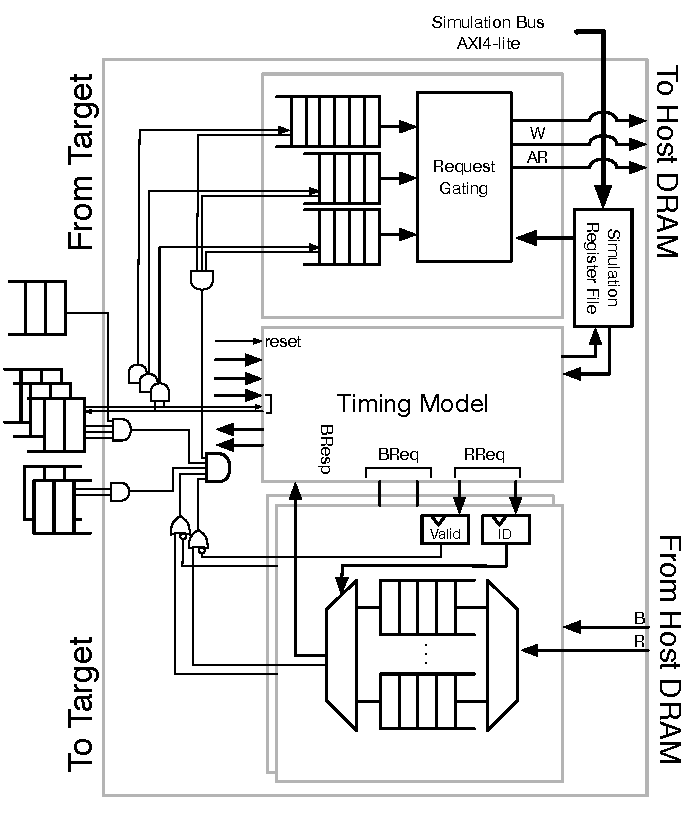
\includegraphics[width=0.99\textwidth]{figures/fased-block-diagram.pdf}
    % graffle2pdf -c full midas-graphics/graffle/memory-model-block-diagram.graffle figures/fased-block-diagram.pdf
    \caption{A timing-model-agnostic block diagram of a FASED memory model with
    all critical control signals.}
    \label{fig:fased-block-diagram}
\end{figure}

How this procedure allows FASED to deterministically model memory system
timings is best illustrated with an example -- to this end, let's consider a
FASED instance us consider modeling a memory system with single cycle of
latency. This is depicted in Figure~\ref{fig:model-operation}.  Suppose we have reached the first
read request issued to the memory system~(Figure~\ref{fig:model-operation-1}). Let this be host and
target cycle 0. When the timing model accepts this request, it is snooped by
host-request scheduler. Simultaneously, the timing model makes a request to
host-response staging module as it needs to reply to the read in the next
target cycle.

In host cycle 2~(Figure~\ref{fig:model-operation-2}), the host-response staging module
cannot produce the associated host response, since it has yet to
be issued, and so generates no fToken, stalling the timing model.
In parallel, the host-request scheduler issues the required read to
the host memory system. While the host-response staging module
waits, the timing model stalls. If the host memory system responds
in K cycles, at host cycle K + 1~(Figure~\ref{fig:model-operation-3}), that response is received.
In cycle K + 2~(Figure~\ref{fig:model-operation-4}), the host-response staging module
produces an output token, targetFire is asserted, and target cycle
1 executes. Here the timing model forwards the data directly into
its output token. From the target’s perspective, the read occurred
in a single cycle, however, the cycle was executed with an FMR of
K + 2. As the latency of the target increases, FMR decreases and
approaches unity. If the target memory system is strictly slower
the host memory system, the instance executes at unity FMR.

\begin{figure*}[t]
    \vspace{-0.25in}
	\centering
    \begin{subfigure}[t]{0.23\textwidth}
        \includegraphics[width=\columnwidth]{figures/model-operation-1.pdf}
        % graffle2pdf -c 1 midas-graphics/graffle/memory-model-operation.graffle figures/model-operation-1.pdf
        \caption{}
        \label{fig:model-operation-1}
    \end{subfigure}
    \begin{subfigure}[t]{0.24\textwidth}
        \includegraphics[width=\columnwidth]{figures/model-operation-2.pdf}
        % graffle2pdf -c 2 midas-graphics/graffle/memory-model-operation.graffle figures/model-operation-2.pdf
        \caption{}
        \label{fig:model-operation-2}
    \end{subfigure}
    \begin{subfigure}[t]{0.24\textwidth}
        \includegraphics[width=\columnwidth]{figures/model-operation-3.pdf}
        % graffle2pdf -c 3 midas-graphics/graffle/memory-model-operation.graffle figures/model-operation-3.pdf
        \caption{}
        \label{fig:model-operation-3}
    \end{subfigure}
    \begin{subfigure}[t]{0.23\textwidth}
        \includegraphics[width=\columnwidth]{figures/model-operation-4.pdf}
        % graffle2pdf -c 4 midas-graphics/graffle/memory-model-operation.graffle figures/model-operation-4.pdf
        \caption{}
        \label{fig:model-operation-4}
    \end{subfigure}
	\centering
    \caption{A FASED instance simulating a single-target-cycle read. Data
    tokens carry target transactions~(their target-valid bit is set) whereas
    empty tokens do not carry a target transaction.}
    \label{fig:model-operation}
\vspace{-0.20in}
\end{figure*}

\subsection{Simulation Performance Case Study}

\begin{table}[t]
\centering
    \begin{tabular}{c@{\hskip 0.1in}
        S[table-format=3.2]@{\hskip 0in}S[table-format=3.2]
        S[table-format=3.2]@{\hskip 0in}S[table-format=3.2]
        S[table-format=3.2]@{\hskip 0in}S[table-format=3.2]}
    \hline
        \textbf{Benchmarks} & \multicolumn{2}{c}{\textbf{Insns~(T)}} & \multicolumn{2}{c}{\textbf{D\$ MPKI}} & \multicolumn{2}{c}{\textbf{I\$ MPKI}} \\
    \hline
        perlbench & 2.98 & 2.99 & 9.0 &  8.9 & 10.0 & 10.1 \\
        gcc & 2.43 & 1.35 & 36.6 & 29.5 & 9.7 &  11.1 \\
        mcf & 1.60 & 0.91 & 97.9 & 80.9 & 0.1 &  0.1 \\
        omnetpp & 1.11 & 1.11 & 56.9 & 56.6 & 9.3 &  10.4 \\
        xalancbmk & 1.21 & 1.21 & 62.9 & 62.9 & 7.9 &  7.6 \\
        x264 & 4.55 & 4.55 & 3.0 &  3.0 & 2.9 &  3.0 \\
        deepsjeng & 2.51 & 2.14 & 8.7 &  8.2 & 15.4 & 15.3 \\
        leela & 2.59 & 2.59 & 5.8 &  5.8 & 1.5 &  1.5 \\
        exchange2 & 3.24 & 3.24 & 0.0 &  0.0 & 0.1 &  0.1 \\
        xz & 9.41 & 2.25 & 19.8 & 15.7 & 0.2 &  0.1 \\
    \hline
    \end{tabular}
    \caption{Dynamic instruction counts and L1 MPKIs of SPEC2017int rate and speed~(single threaded), respectively.}
    \label{tbl:spec-insns}
\vspace{-0.35in}
\end{table}

\subsubsection{Target Designs}\label{sec:target-parameters} Our target designs
are derived from the Rocket Chip generator~\cite{rocketchip}, which contains
Rocket, a single-issue in-order scalar core implementing the RISC-V
ISA~(RV64IMAFDC). Rocket Chip
has been taped out over a dozen times for both research and commercial
purposes. In our
experiments, we use the default
configuration of Rocket Chip, which includes
a \wunits{16}{KiB} L1 I\$, a blocking \wunits{16}{KiB} L1 D\$, and 32-entry
fully-associative L1 I and D TLBs. We only change the default configuration to
increase the number of performance counters and deepen the L2 TLB to 1024 entries.

At the system level, our targets consist of single or quad-core instances
of Rocket Chip (labeled SC or QC), composed with either a latency-bandwidth pipe
or a quadruple-rank DDR3-2133~(14-14-14) FCFS or FR-FCFS
DRAM models over a 64-bit AXI4 bus. In all targets, the simulated system has
16 GiB of DRAM capacity. Additionally, two targets include a 4 MiB
LLC model~(labeled LLC). In the target's periphery, we have a UART and block
device that interact with simulation models co-hosted in software.

\subsection{An Overview SPEC2017int On Rocket}
In our experiments, we run SPEC2017 intrate and intspeed suites with reference
inputs, cross-compiled for RISC-V systems with the \texttt{-O2} flag.
Intspeed benchmarks require as much as \wunits{16}{GB} of memory, while intrate
benchmarks require \wunits{2}{GB} per copy.  In Table~\ref{tbl:spec-insns}, we give each suite's dynamic instruction
count and L1 MPKIs when running on the Rocket configuration of
Section~\ref{sec:target-parameters}

\input{tex/tables/simulator-performance.tex}

Table~\ref{tbl:intrate-simtimes} gives the
host-execution times and execution speeds for a handful of SPEC2017 runs. The
targets with DDR3 models consistently run at rates above \wunits{100}{MHz}. Theoretically,
FASED instances can operate at the host frequency~(160 MHz) if the functional model can always serve timing model requests in time.
On our host, reads and writes take on average 47
and 37 cycles, respectively, when unloaded.  These latencies have
a significant effect on simulator performance when modeling a single-cycle memory
system as that host latency is fully exposed to the simulator, but
they have relatively little impact
when modeling a realistic DRAM system
whose latency~(cycles) is similar to that of the host.
Instances with LLCs fall between these extremes: LLC hits are fast in
target time and thus expose the host-DRAM latency to simulator, while
misses present sufficient target-latency to hide the host-DRAM access.
For our DDR3-2133 target memory system, reads take 20, 34, and 48 cycles for
row hits, closed row, and row misses, respectively. These latencies are large enough that many accesses can be
served by the functional model before the timing model requires them, eliding simulator stalls.
Ironically, modeling a slower DDR-speed-grade slows down the simulator: since $t_{CS}$ is smaller, reads complete in fewer target
\emph{cycles} despite taking more target \emph{time}.

\subsection{Limitations}
The downside of this approach is that FASED replaces the target memory
controller, whereas a device-based model does not. Thus, while FASED provides a
more accurate model of DRAM memory timings they will not match that of the ASIC
memory controller, and could possibly differ wildly, if their memory access
schedulers are substantially different. One way to ameloirate this, is to
instantiate ASIC DRAM controller directly within a new FASED memory timing
model\footnote{In the future we plan make this easier by breaking FASED into
two libaries -- an inline, AXI4-memory slave bridge, which can be inserted
between any AXI4 master and slave, and a library of timing models that can be
instantiated in the target design these timing models will expose their
configuration and instrumentation registers to a second bridge. Users who wish
to simulate their own memory controllers can then instantiate just the
functional model.} While this will produce timings that exactly match that of
desired memory system, FASED's functional model can still mask datapath bugs in
the DRAM controller RTL since the functional model will always return correct
data, where as a device-based model would correctly simulate the erroneous
behavior.

